\documentclass[conference,a4paper]{IEEEtran}

\usepackage[utf8]{inputenc}
\usepackage[T1]{fontenc}
\usepackage[english]{babel}
\usepackage{cite}
\usepackage{amsmath}
\usepackage{booktabs}
\usepackage{array}
\usepackage{graphicx}
\usepackage{tikz}
\usepackage{url}
\usepackage{xcolor}
\usepackage{balance}
\usepackage{xspace}
\usepackage[hidelinks]{hyperref}

\hypersetup{
    pdftitle={ArGos: A Scope-Constrained and Evidence-Oriented EASM Platform with Multi-Provider LLM and MCP Integration},
    pdfauthor={Ruben Torres},
    pdfkeywords={attack surface management, vulnerability verification, cybersecurity automation, large language models, Model Context Protocol}
}

\usetikzlibrary{arrows.meta,positioning,fit,shapes.geometric}
\newcommand{\argos}{ArGos\xspace}
\newcommand{\code}[1]{\texttt{#1}}

\title{\argos: A Scope-Constrained and Evidence-Oriented EASM Platform\\
with Multi-Provider LLM and MCP Integration}

\author{
\IEEEauthorblockN{Rub\'en Torres, \textit{Member, IEEE}}
\IEEEauthorblockA{\textit{Research Department}\\
\textit{STEAM Robotics Academy}\\
San Salvador, El Salvador\\
rtorres.plus25@gmail.com}
\and
\IEEEauthorblockN{Edwin Henriquez}
\IEEEauthorblockA{\textit{Independent Researcher}\\
San Salvador, El Salvador\\
ehciberseguridad@gmail.com}
\and
\IEEEauthorblockN{Bryan V\'asquez-Pineda, \textit{Member, IEEE}}
\IEEEauthorblockA{\textit{Research Department}\\
\textit{STEAM Robotics Academy}\\
San Salvador, El Salvador\\
cawy.288@gmail.com}
}

\begin{document}

\maketitle

\begin{abstract}
External attack surface management (EASM) joins asset discovery, service probing, vulnerability detection, prioritization, and reporting, but its automation creates two practical risks: scanners may leave the authorized perimeter, and unverified detections may be presented as facts. Language-model assistance adds a third risk because attacker-controlled banners, hostnames, and findings can become indirect prompt-injection inputs. This paper presents \argos, an EASM platform that treats authorization, evidence, and tenant isolation as first-class system properties. A Go worker orchestrates subdomain discovery, port and HTTP probing, TLS inspection, signature-based scanning, optional dynamic application security testing, and repeated oracle-based verification. A deterministic Cyber Score exposes the penalty breakdown separately from the natural-language explanation. Tenant-scoped data tools are available both to an integrated agent and through a Streamable HTTP Model Context Protocol (MCP) server. The language-model layer supports native OpenAI, Anthropic, and Gemini protocols while preserving tool calls, streaming, token accounting, and provider-specific reasoning metadata. Artifact-level validation produced 298 passing Go test events across 30 packages and 36 passing frontend tests; static analysis, Docker Compose validation, and race-enabled tests over eight security-critical packages also completed without failures. These results establish implementation consistency and enforcement of key invariants, not vulnerability-detection accuracy. The remaining empirical gaps---large-scale scan recall, false-positive reduction in live targets, and adversarial evaluation of the LLM boundary---are stated explicitly as future evaluation requirements.
\end{abstract}

\begin{IEEEkeywords}
attack surface management, vulnerability verification, cybersecurity automation, large language models, Model Context Protocol.
\end{IEEEkeywords}

\section{Introduction}

Internet-facing infrastructure changes continuously as teams add subdomains, deploy services, rotate certificates, and expose administrative interfaces. Fast scanning systems such as ZMap demonstrated that Internet-wide measurement can be practical~\cite{Durumeric2013ZMap}; Censys subsequently showed how repeated scanning can support a searchable view of public services~\cite{Durumeric2015Censys}. Enterprise EASM narrows that capability to the assets an organization is authorized to assess and adds prioritization, historical comparison, and remediation support.

The engineering problem is not only to run scanners. First, discovery can produce third-party hosts or redirects, so authorization must be enforced again at execution time rather than assumed from an initial target string. Second, signature-based findings are observations, not automatically verified vulnerabilities. Third, severity alone is an incomplete remediation signal. The limitations of a single Common Vulnerability Scoring System (CVSS) value have been discussed since early empirical analyses~\cite{Mell2006CVSS,Scarfone2009CVSS}, while the Exploit Prediction Scoring System (EPSS) and recent prioritization surveys emphasize exploitation probability, context, and multiple evidence sources~\cite{Jacobs2021EPSS,Jiang2025Prioritization}. Finally, an LLM that reads scan output is exposed to text controlled by the scanned system. Indirect prompt injection can convert retrieved content into adversarial instructions~\cite{Greshake2023Indirect,Hines2024Spotlighting}.

\argos addresses these concerns as an integrated system rather than as independent wrappers around security tools. Its design separates deterministic security state from generated explanation, carries tenant identity through every read path, and places explicit authorization gates before active operations. The platform also exposes a model-independent tool surface through MCP, whose interoperability benefits and security risks are the subject of active research~\cite{Hou2025MCP,Hasan2026MCP}.

This paper makes four contributions:
\begin{itemize}
    \item A scope-constrained EASM pipeline that composes asset discovery, service and TLS inspection, vulnerability scanning, optional DAST, and fail-open enrichment while keeping core stages fail-closed.
    \item An evidence-oriented finding model that distinguishes candidates from findings verified through repeated, class-specific oracles and stores portable verification receipts.
    \item A tenant-scoped LLM and MCP boundary that combines tool authorization, execution tracking, token accounting, and explicit delimitation of untrusted scan content.
    \item An artifact-level evaluation of the implemented invariants, including unit, integration, race, frontend, static-analysis, and deployment-configuration checks.
\end{itemize}

The contribution is therefore a system architecture and implementation artifact. It is not a claim that \argos outperforms existing scanners in recall or that its current deterministic score supersedes CVSS or EPSS.

\section{Related Work}

\subsection{Discovery and vulnerability scanning}

ZMap introduced a stateless approach to high-speed network scanning and also discussed responsible measurement practices~\cite{Durumeric2013ZMap}. The Censys architecture transformed repeated protocol scans into structured, searchable service data~\cite{Durumeric2015Censys}. These systems motivate scalable discovery, whereas \argos focuses on organization-scoped execution, longitudinal scan records, and analyst-facing interpretation. Web vulnerability scanners commonly combine crawling, request generation, and response analysis~\cite{Chen2020WebScanner}. Recent work has also explored adding AI to specific web-vulnerability classes~\cite{Manivannan2025AIScanner}; \argos instead keeps detection and verification deterministic and uses the LLM for tool selection and explanation.

\subsection{Risk prioritization}

CVSS provides a shared severity vocabulary, but its score is not a direct estimate of exploitation in a particular environment~\cite{Mell2006CVSS,Scarfone2009CVSS}. EPSS introduced a data-driven probability of exploitation and reported better prioritization utility than severity-only practice~\cite{Jacobs2021EPSS}. A recent survey organizes vulnerability prioritization by severity, exploitability, context, and aggregation strategy~\cite{Jiang2025Prioritization}; vulnerability-management chaining likewise combines CVSS, EPSS, and known-exploited signals~\cite{Shimizu2025Chaining}. \argos currently uses a transparent, deterministic penalty model so an executive grade is reproducible. Incorporating EPSS, known-exploited-vulnerability data, and asset criticality is future work, not an implemented claim.

\subsection{LLMs, agents, and MCP in security operations}

ReAct interleaves reasoning and external actions, providing a general pattern for tool-using language agents~\cite{Yao2023ReAct}. Surveys of LLM-assisted security operations identify alert triage, vulnerability management, summarization, and reporting as promising tasks, while also emphasizing hallucination, privacy, and adversarial robustness~\cite{Habibzadeh2025LLMSOC,Srinivas2025AISOC}. Prompt injection is especially relevant when security telemetry includes attacker-controlled strings~\cite{Greshake2023Indirect}. Spotlighting proposes explicit transformations or delimiters for untrusted content~\cite{Hines2024Spotlighting}; security-specific guardrail research further argues for layered controls and continual red-teaming~\cite{Ali2026SecureCAI}.

MCP standardizes discovery and invocation of model-accessible tools. Its open interface reduces provider coupling but creates distinct lifecycle and tool-poisoning risks~\cite{Hou2025MCP}. An empirical study of 1,899 open-source MCP servers found both conventional vulnerabilities and MCP-specific weaknesses~\cite{Hasan2026MCP}. These findings motivate \argos' narrow schemas, per-tool authorization, tenant-derived scope, and audit records.

\section{System Goals and Threat Model}

\argos assumes that an authenticated tenant operator may scan only verified domains or explicitly allowlisted laboratory networks. Discovered hosts, redirect destinations, HTTP content, certificate metadata, template names, and vulnerability descriptions are untrusted. An API token can be stolen or over-privileged; therefore authentication alone is insufficient and each tool requires an authorization decision. LLM providers are treated as external processors: model output may be incorrect and provider protocols may differ.

The design follows five goals:
\begin{enumerate}
    \item \textit{Fail-closed scope}: malformed, excluded, or unmatched targets are denied before a scanner process is invoked.
    \item \textit{Evidence separation}: a detector creates a candidate; only a successful oracle promotes it to verified.
    \item \textit{Deterministic security state}: scores and raw findings do not depend on an LLM response.
    \item \textit{Tenant-derived access}: tenant identifiers come from authenticated identity, never from model-supplied tool arguments.
    \item \textit{Provider portability}: vendor-specific message, tool, streaming, reasoning, and usage formats remain behind one interface.
\end{enumerate}

The current threat model does not defend against compromise of the host running the worker, malicious scanner binaries, or a fully compromised database administrator. It also does not prove that delimiting untrusted text defeats all prompt-injection attacks.

\section{Architecture and Implementation}

Fig.~\ref{fig:architecture} shows the control and data paths. The Vue client calls a Go HTTP control plane. Scan jobs are executed by a separate Go worker, allowing scan concurrency and network egress to be isolated from the API. PostgreSQL stores tenant-scoped targets, scans, findings, evidence, scores, chat history, token usage, and MCP audit records. The integrated assistant and the MCP server share domain stores and the same LLM-provider registry.

\begin{figure*}[t]
\centering
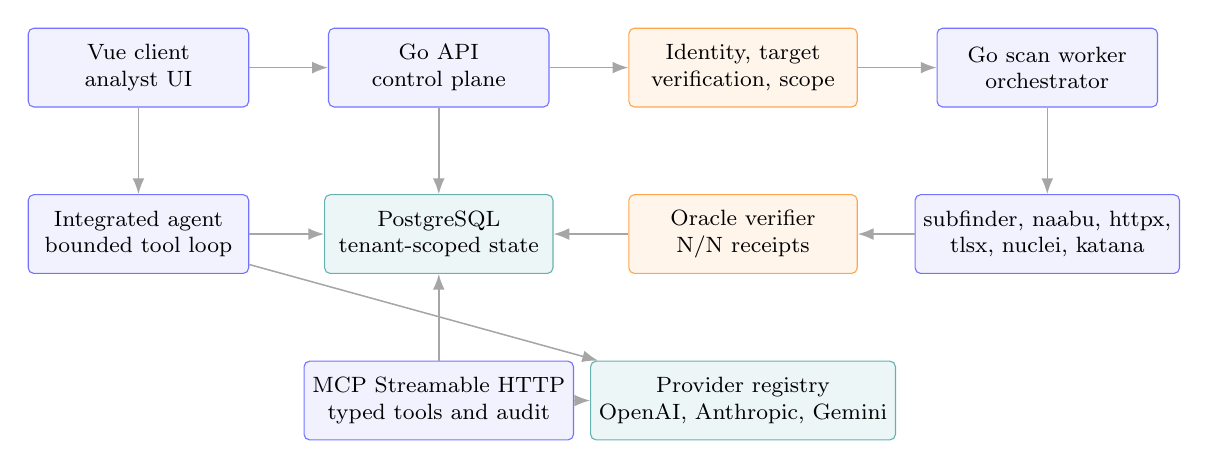
\begin{tikzpicture}[
    font=\footnotesize,
    node distance=7mm and 10mm,
    box/.style={draw=blue!55, rounded corners=2pt, fill=blue!5, align=center,
                minimum width=28mm, minimum height=10mm, inner sep=3pt},
    sec/.style={draw=orange!70, rounded corners=2pt, fill=orange!8, align=center,
                minimum width=29mm, minimum height=10mm, inner sep=3pt},
    data/.style={draw=teal!60, rounded corners=2pt, fill=teal!7, align=center,
                 minimum width=29mm, minimum height=10mm, inner sep=3pt},
    flow/.style={-{Latex[length=2mm]}, line width=0.55pt, draw=gray!70}
]
\node[box] (ui) {Vue client\\analyst UI};
\node[box, right=of ui] (api) {Go API\\control plane};
\node[sec, right=of api] (scope) {Identity, target\\verification, scope};
\node[box, right=of scope] (worker) {Go scan worker\\orchestrator};

\node[data, below=11mm of api] (db) {PostgreSQL\\tenant-scoped state};
\node[sec, below=11mm of scope] (verify) {Oracle verifier\\N/N receipts};
\node[box, below=11mm of worker] (tools) {subfinder, naabu, httpx,\\tlsx, nuclei, katana};

\node[box, below=11mm of ui] (agent) {Integrated agent\\bounded tool loop};
\node[box, below=11mm of db] (mcp) {MCP Streamable HTTP\\typed tools and audit};
\node[data, below=11mm of verify] (llm) {Provider registry\\OpenAI, Anthropic, Gemini};

\draw[flow] (ui) -- (api);
\draw[flow] (api) -- (scope);
\draw[flow] (scope) -- (worker);
\draw[flow] (worker) -- (tools);
\draw[flow] (tools) -- (verify);
\draw[flow] (verify) -- (db);
\draw[flow] (api) -- (db);
\draw[flow] (agent) -- (db);
\draw[flow] (mcp) -- (db);
\draw[flow] (agent) -- (llm);
\draw[flow] (mcp) -- (llm);
\draw[flow] (ui) -- (agent);
\end{tikzpicture}
\caption{\argos architecture. Authorization precedes active scanning; deterministic findings, evidence, and scores are persisted before optional LLM explanation.}
\label{fig:architecture}
\end{figure*}

\subsection{Scope-constrained scan pipeline}

The scope enforcer accepts exact domains, wildcard apexes, CIDRs, and a separate laboratory CIDR allowlist. Explicit domain and network exclusions take precedence. DNS resolution is disabled by default; if enabled, all resolved addresses are checked against exclusions and allowed networks. The ProjectDiscovery adapters repeat the scope check immediately before process execution. This second check is important because the pipeline may receive hosts from discovery and crawling rather than directly from the user.

The worker executes the following stages:
\begin{equation}
\begin{split}
\mathrm{target} &\rightarrow \mathrm{subdomains} \rightarrow \mathrm{ports} \\
&\rightarrow \mathrm{HTTP} \rightarrow \mathrm{TLS} \rightarrow \mathrm{nuclei} \\
&\rightarrow [\mathrm{crawl} \rightarrow \mathrm{DAST}] \rightarrow [\mathrm{verify}].
\end{split}
\label{eq:pipeline}
\end{equation}
Subdomain enumeration, HTTP probing, and signature scanning are core stages. Port and TLS inspection, DAST, and oracle verification are enrichment stages: a local failure is recorded and the scan can continue unless the context is cancelled. DAST is opt-in because it injects payloads. Host limits, request-rate profiles, timeouts, and cancellation provide resource guardrails.

\subsection{Evidence-oriented verification}

Each finding receives a stable fingerprint derived from normalized identifying fields. The verifier maps supported template signals to one of 26 oracle classes, including exposed panels, directory listing, CORS, unsafe HTTP methods, reflected or stored XSS, SQL injection variants, SSRF, XXE, JWT \code{alg:none}, IDOR, HTTP desynchronization, type confusion, and mass assignment. Intrusive classes require both DAST opt-in and an in-scope target.

An oracle repeats an idempotent check $N$ times, where $N=2$, $3$, or $5$ for stealth, normal, or aggressive profiles. A candidate is promoted only when
\begin{equation}
    \mathrm{verified}(f) \iff \mathrm{successes}(f)=\mathrm{attempts}(f)>0.
\end{equation}
Technical errors do not refute a finding; they leave it as a candidate. A successful verification stores the redacted recipe, request/response evidence, attempt count, oracle type, and fingerprint. This receipt supports later audit and re-verification without asking an LLM to judge exploitability.

\subsection{Transparent scoring}

The Cyber Score converts the current scan into a number and letter while preserving its breakdown. Let $F$ be the findings and $C$ the observed certificates. The current implementation computes
\begin{equation}
S=\max\left(0,100-\sum_{f\in F}w(s_f)-\sum_{c\in C}t(c)\right),
\end{equation}
where $w$ assigns penalties 40, 20, 8, 3, and 1 to critical, high, medium, low, and informational findings. The TLS function assigns 15 to an expired certificate and 10 each to a self-signed certificate or obsolete SSL/TLS version. Grades A--F correspond to thresholds 90, 80, 70, 60, and 50. This model is intentionally simple and explainable; the interface displays both $S$ and the penalty components. It should not be interpreted as an exploitation probability.

\subsection{Tenant-aware agent and MCP surface}

The assistant uses a bounded tool loop with at most five LLM iterations. Tools list domains and scans, retrieve overviews, filter findings, and inspect ports and TLS issues. Results are inserted into the model context with an explicit marker stating that scan data is untrusted and must not be treated as instructions. This is a datamarking defense inspired by spotlighting~\cite{Hines2024Spotlighting}, but the system does not claim formal resistance to adaptive attacks.

The MCP server exposes the same tenant-scoped concepts through typed tools. Bearer API keys are stored as hashes and resolve to an identity containing tenant, token, and scopes. Authorization middleware runs per tool call; execution tracking stores an argument digest, outcome, latency, and result size. Read-only annotations are applied to data tools, while expert escalation is explicitly marked as state-changing. Cross-tenant scans return no data even if a model supplies another scan identifier.

\subsection{Native multi-provider LLM layer}

One provider interface covers synchronous chat, streaming, tool definitions, tool calls, and token usage. A thread-safe factory atomically replaces the active provider set when environment fallbacks or encrypted database configuration change. OpenAI-compatible endpoints use the chat-completions contract. Anthropic and Gemini use native message, tool, streaming, usage, and reasoning structures; catalog identifiers are translated to exact API model identifiers. Provider metadata retains Anthropic thinking signatures and Gemini thought signatures across tool round trips. The interface records prompt and completion usage without making generated text part of the Cyber Score.

\section{Operational Interface}

The interface presents the deterministic scan state before generated interpretation. Fig.~\ref{fig:ui-analysis} shows a scan record and an assistant response over the same operational data. The screenshots are demonstration artifacts, not quantitative experiment results.

\begin{figure*}[t]
    \centering
    \begin{minipage}[t]{0.49\textwidth}
        \centering
        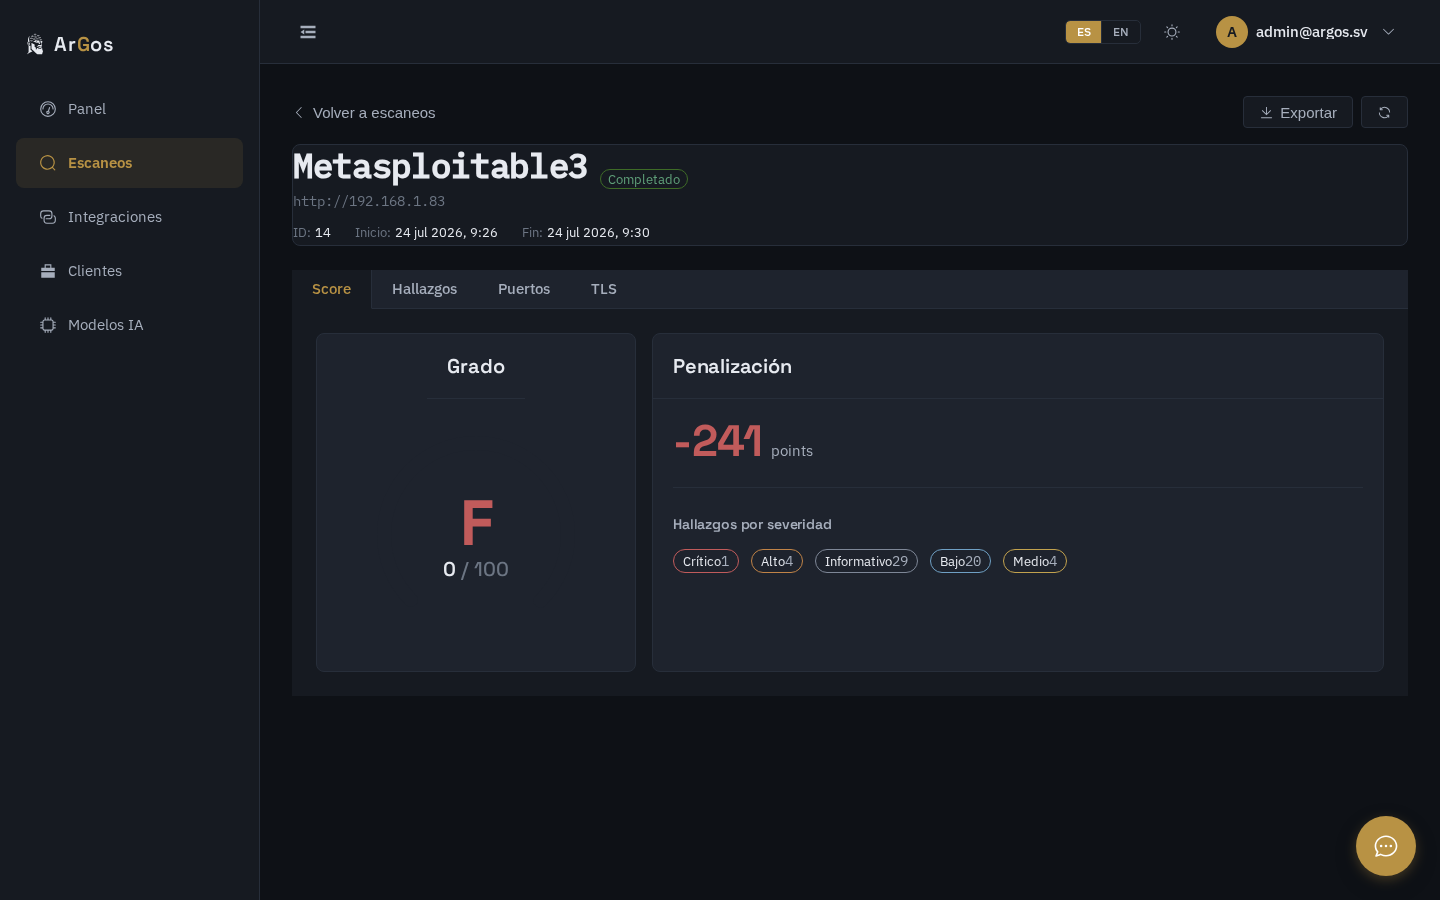
\includegraphics[width=\linewidth]{figures/scan-detail.png}
        \small (a) Scan detail with grade and penalty breakdown.
    \end{minipage}
    \hfill
    \begin{minipage}[t]{0.49\textwidth}
        \centering
        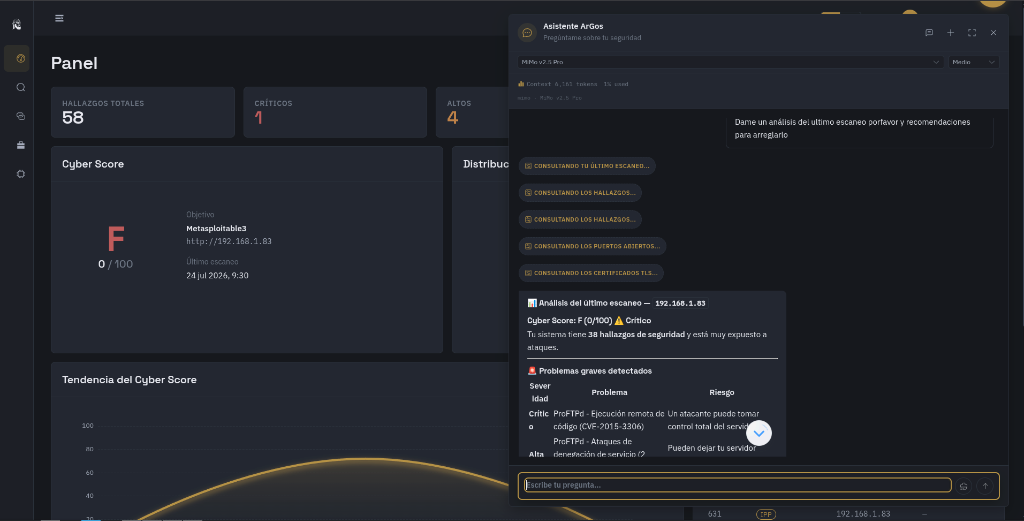
\includegraphics[width=\linewidth]{figures/chatbot-response.png}
        \small (b) Tool-assisted explanation displayed beside scan context.
    \end{minipage}
    \caption{Analyst workflow in the \argos demonstration. Generated explanation augments, but does not replace, persisted findings and score components.}
    \label{fig:ui-analysis}
\end{figure*}

Fig.~\ref{fig:ui-governance} illustrates two governance boundaries: provider configuration is an administrative function, and a tenant dashboard exposes only organization-scoped state. The UI can switch language and theme, but those presentation options do not alter authorization.

\begin{figure*}[t]
    \centering
    \begin{minipage}[t]{0.49\textwidth}
        \centering
        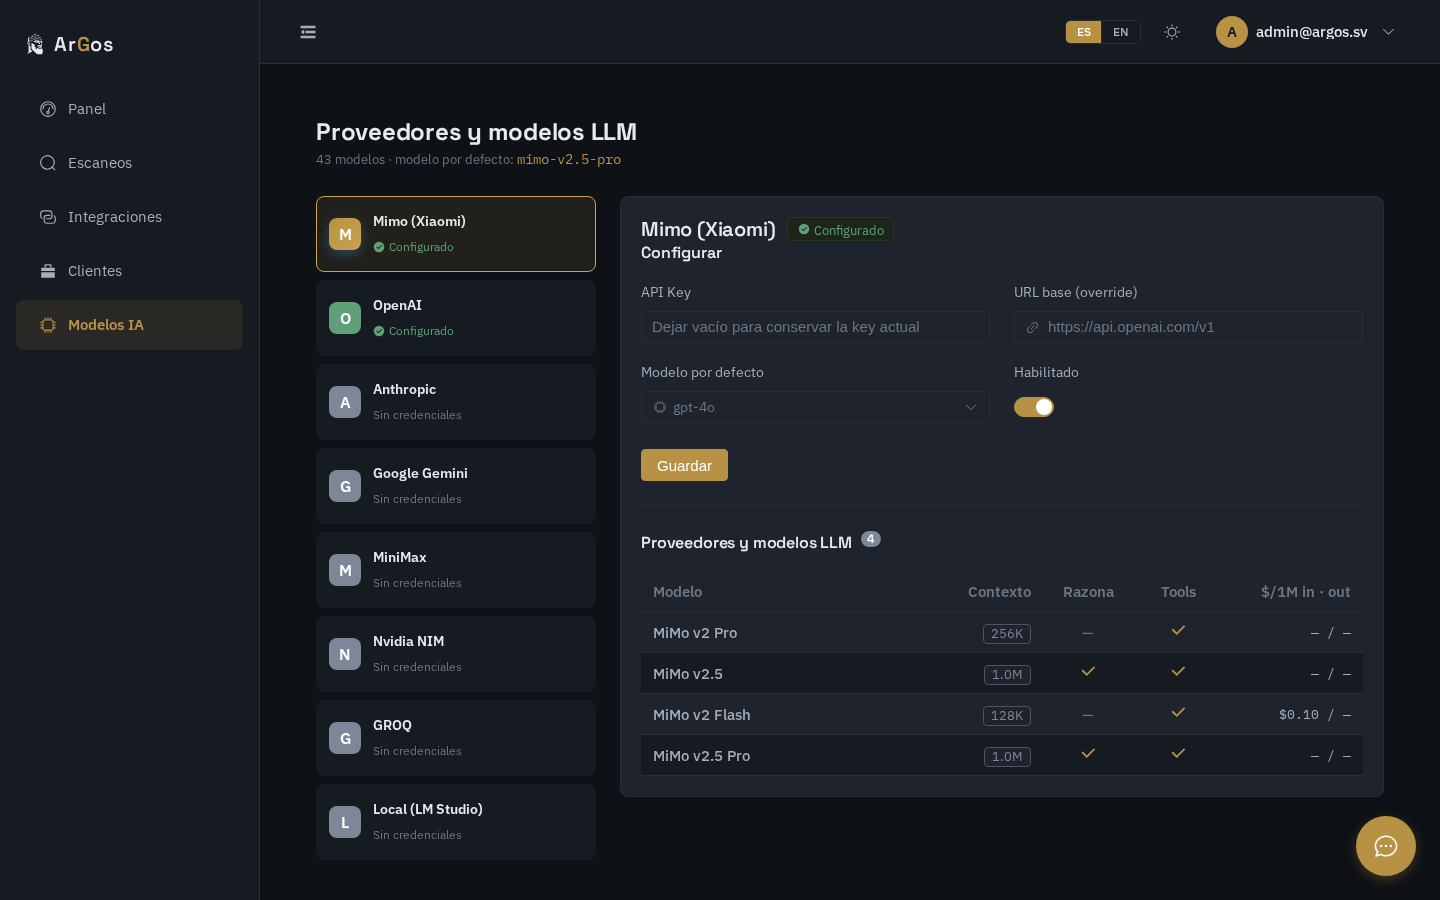
\includegraphics[width=\linewidth]{figures/ai-providers.png}
        \small (a) Administrative provider and model configuration.
    \end{minipage}
    \hfill
    \begin{minipage}[t]{0.49\textwidth}
        \centering
        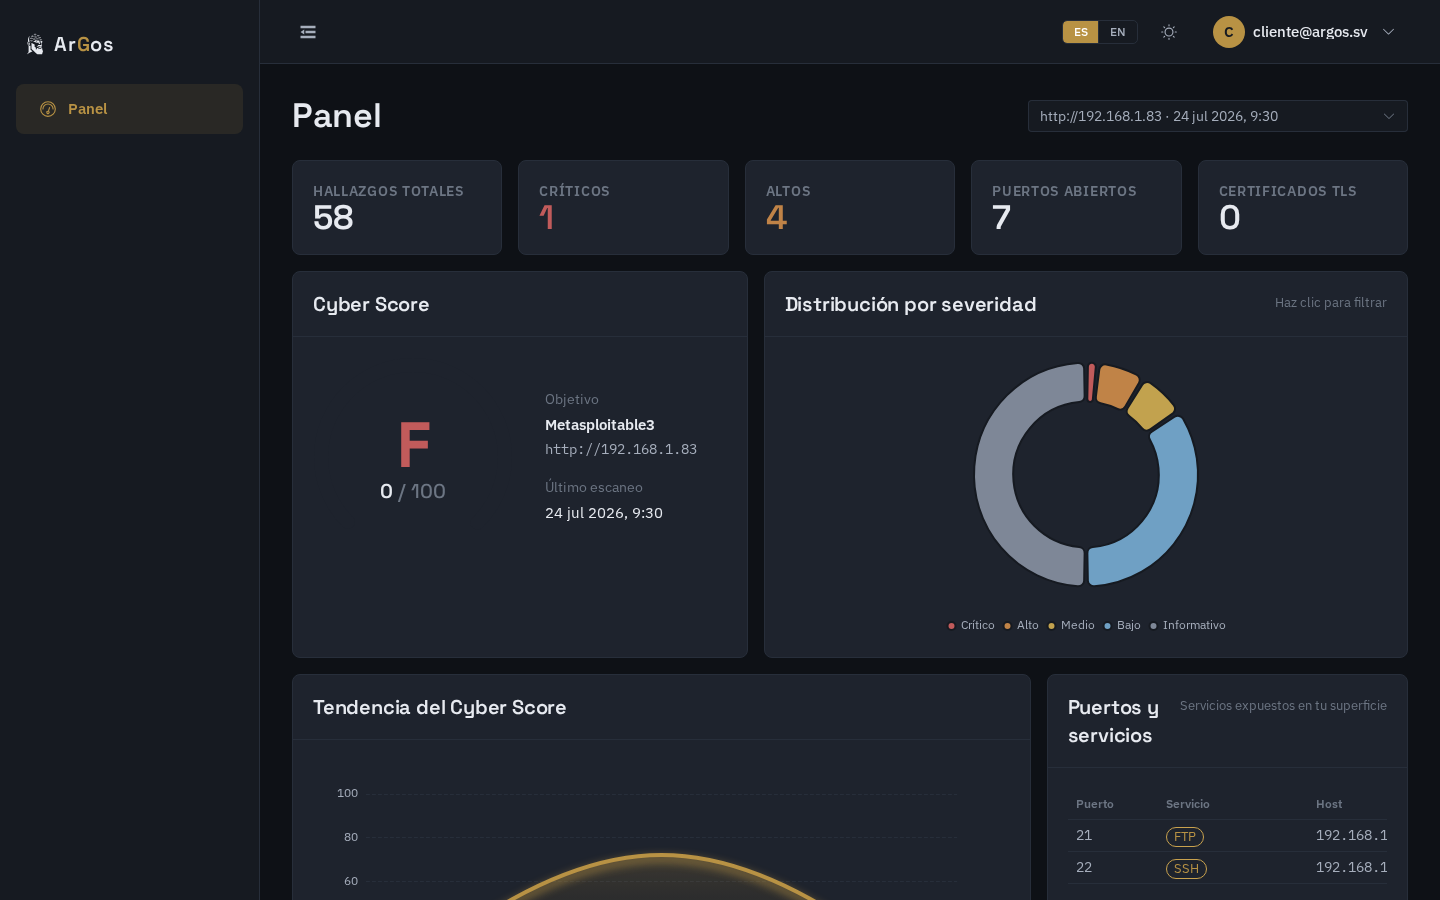
\includegraphics[width=\linewidth]{figures/tenant-dashboard.png}
        \small (b) Tenant-restricted posture dashboard.
    \end{minipage}
    \caption{Provider governance and tenant isolation in the web interface. API credentials are not returned to the frontend after persistence.}
    \label{fig:ui-governance}
\end{figure*}

\section{Evaluation}

\subsection{Research questions}

The evaluation asks four artifact-level questions: \textbf{RQ1}: do scope and tenant boundaries reject unauthorized inputs? \textbf{RQ2}: do oracle and evidence components preserve the candidate/verified distinction? \textbf{RQ3}: do MCP and provider adapters preserve authorization, native protocol semantics, streaming, tools, and usage? \textbf{RQ4}: does the complete repository pass its automated quality gates?

\subsection{Environment and procedure}

The evaluation used Linux 7.1.5 on x86-64, Go 1.26.5, Node.js 26.4.0, pnpm 11.9.0, and Vitest 4.1.9. The evaluated working tree was based on commit \code{71f8bd4}. Backend tests were run with \code{go test -json ./\ldots}; the number reported is the count of passing Go test events, including named subtests, rather than a claim of 298 independent security properties. Security-critical packages were then rerun with Go's race detector. The frontend suite was run once in non-watch mode. Static analysis and deployment syntax were checked with \code{go vet ./\ldots} and \code{docker compose config --quiet}.

\begin{table}[t]
\centering
\caption{Automated validation summary}
\label{tab:validation}
\begin{tabular}{p{0.32\columnwidth}p{0.43\columnwidth}r}
\toprule
Layer & Validation focus & Passed \\
\midrule
Oracle & Differential checks and evidence & 62 \\
HTTP API & Auth, handlers, provider refresh & 22 \\
LLM adapters & Native requests, streams, tools, usage & 22 \\
Scope & Domain, CIDR, exclusion, DNS behavior & 21 \\
Scan & Pipeline, cancellation, deduplication & 20 \\
Evidence & Capture, hashing, integrity & 12 \\
MCP & Auth, scoping, pagination, HTTP transport & 12 \\
Other Go packages & Domain and adapter behavior & 127 \\
Vue frontend & Components and API client & 36 \\
\midrule
Total & Go test events plus frontend tests & 334 \\
\bottomrule
\end{tabular}
\end{table}

All 298 Go test events passed across 30 packages with zero failed events. All 36 frontend tests in six files passed. Table~\ref{tab:validation} breaks out the packages most relevant to the paper; the remaining Go packages include knowledge retrieval, API keys, governance, orchestration, exports, and execution adapters.

\begin{table}[t]
\centering
\caption{Invariant-oriented checks}
\label{tab:invariants}
\begin{tabular}{p{0.29\columnwidth}p{0.57\columnwidth}}
\toprule
Invariant & Representative automated check \\
\midrule
Scope confinement & Exact/wildcard/CIDR matching, exclusion precedence, unresolved and malformed targets, scoped scanner adapters. \\
Tenant isolation & Cross-tenant MCP overview rejected; tenant domain lists cannot expose another tenant. \\
Evidence boundary & Out-of-scope and non-repeatable candidates are not promoted; verified findings retain receipts. \\
DAST gate & Intrusive oracle classes require explicit DAST enablement. \\
MCP authentication & Missing bearer key rejected; generated key lists tools over Streamable HTTP. \\
Provider semantics & Native Anthropic/Gemini tool calls, streaming usage, reasoning signatures, and model dispatch checked against mock HTTP contracts. \\
\bottomrule
\end{tabular}
\end{table}

Race-enabled tests passed for scope, scoring, scan, verifier, oracle, MCP, LLM, and assistant packages. \code{go vet} reported no findings, and Docker Compose configuration validation succeeded. These results answer RQ1--RQ4 at the implementation level: the tested invariants hold for the encoded cases and mock protocol contracts.

\subsection{What the evaluation does not establish}

The validation does not compare \argos against commercial EASM products, estimate discovery recall, or measure false-positive reduction on a representative live corpus. It does not make real paid API calls to OpenAI, Anthropic, or Gemini; provider tests use controlled HTTP servers that assert the documented native request and stream shapes. It also does not evaluate whether a language model answers MCP task sets correctly or withstands adaptive prompt injection. These distinctions prevent passing software tests from being misreported as security effectiveness.

\section{Discussion}

The architecture demonstrates a useful separation of responsibilities. Deterministic components decide scope, collect evidence, and compute the score; the LLM selects read tools and converts persisted state into language. This reduces the consequence of hallucination because a generated explanation cannot silently mutate the underlying grade or verified verdict. Provider-native adapters also avoid forcing vendor APIs through an OpenAI-compatible approximation, which is important for tool-call signatures and token accounting.

The verifier's N/N rule favors precision and auditability over aggressive promotion. Its principal weakness is coverage: unsupported findings remain candidates, and a deterministic oracle can still encode an incomplete condition. Receipts make that limitation inspectable but do not remove it. Similarly, the Cyber Score is transparent but presently omits exploitation probability, asset criticality, exposure duration, and compensating controls. The prioritization literature suggests that these signals should be added as separate, attributable factors rather than hidden inside generated prose~\cite{Jacobs2021EPSS,Jiang2025Prioritization,Shimizu2025Chaining}.

MCP creates an explicit tool boundary, but tool descriptions, schemas, dependencies, and returned content remain attack surfaces~\cite{Hou2025MCP,Hasan2026MCP}. \argos mitigates some of these risks through narrow tool sets, scope-derived identity, audit, and untrusted-data marking. Future red-team evaluation should include malicious hostnames, vulnerability descriptions, stored scan evidence, tool-call argument manipulation, and compromised provider responses.

\section{Limitations and Threats to Validity}

\textit{Construct validity}: passing tests measure conformance to encoded behavior, not vulnerability-detection accuracy or operational risk reduction. The score's A--F output is an internal management abstraction rather than a standardized metric.

\textit{Internal validity}: mock HTTP servers isolate provider contracts but cannot capture all production API changes, rate limits, or network behavior. Test-event counts include subtests and are reported as such. Screenshots contain demonstration data and are not treated as experimental measurements.

\textit{External validity}: the artifact has not yet been benchmarked across diverse enterprise domains, cloud providers, network conditions, or scanner versions. Laboratory targets such as OWASP Juice Shop, DVWA, and Metasploitable3 are intentionally vulnerable and do not represent production prevalence.

\textit{Security validity}: scope checks and DAST gates reduce accidental overreach but do not replace legal authorization or operational change control. Datamarking is only one layer against prompt injection, and no universal defense is claimed.

\section{Conclusion and Future Work}

This paper presented \argos, a scope-constrained, evidence-oriented EASM platform that integrates deterministic scanning and scoring with tenant-aware LLM and MCP interfaces. The implementation enforces authorization before active execution, separates candidate from verified findings through repeated oracles, and keeps generated explanation outside the source of truth. Native OpenAI, Anthropic, and Gemini adapters preserve vendor-specific tool and usage semantics behind one provider interface. Automated validation passed across backend, frontend, race, static-analysis, and deployment-configuration checks.

The next evaluation phase should run controlled longitudinal scans over owned targets and report asset-discovery recall, finding precision, verification yield, runtime, and request volume by intensity profile. Prioritization should incorporate EPSS, known-exploited-vulnerability signals, asset criticality, and temporal exposure as separately visible factors. The MCP layer should be evaluated with stable multi-tool question sets and adversarial prompt-injection corpora. Finally, live-provider conformance tests should complement mock contracts while redacting tenant data and controlling cost.

\section*{Artifact Availability}

The repository contains the Go backend, Vue frontend, OpenAPI contract, database migrations, Docker Compose laboratory, tests, screenshots, and the LaTeX source of this paper. The reviewed research PDFs are retained locally as research material and are excluded from product releases.

\section*{Acknowledgment}

The author thanks the maintainers of ProjectDiscovery's scanning tools and the researchers whose openly available papers informed the design and limitations analysis.

\balance
\bibliographystyle{IEEEtran}
\bibliography{references}

\end{document}
